\subsection{Context}

\subsubsection{Introduction}

Computational science is a growing field that allows researchers to predict the behaviour of systems. For example, a physicist can write a program to predict the trajectory of a sphere instead of calculating it by hand.

 What if we bring this further?  We can try to optimize the aero-dynamism of a plane to save fuel, the behaviour of the human body cells to a recently designed drug or even given a genome figure out the risk of cancer.

Computing these are at a high cost. It is not conceivable to solve the problems on our laptops as the number of calculations and data required to process is overwhelming. To solve these tasks, we need supercomputers.

Supercomputers are machines with a huge compute power oriented to scientific and technique jobs. These machines are many small machines interconnected. Developers must write their code in a manner that the program is capable of run in parallel. 

Writing efficient parallel programs is a difficult task and even more so if the developer's specialization is not computer science. In this work, we will study and improve Alya \cite{alya}, a real use case application. In particular, we will focus on the module in charge of computing combustion processes.


This work is under an Educational Cooperation Agreement between the Facultat d'Informàtica de Barcelona and the Barcelona Supercomputing Center.

The study has been developed within a Curricular internship in the Barcelona Supercomputing Center precisely in the High-Level Support Team (HLST) inside the Operations department and developed under a collaboration with the Best Practices for Performance and Programmability group. This work is impulsed by the Performance Optimization and Productivity \cite{popWeb} (POP) Center of Excellence under a  Performance Analysis request.

\subsubsection{Terms and concepts}
In the following sections you will find basic concepts to better understand the project.

\textbf{High-performance computing}

High-performance computing (HPC) refers to the act of grouping compute power to do massive and complex computations and data processing. Nowadays HPC is associated to supercomputers.

\textbf{Supercomputer}

A supercomputer is a machine designed for HPC. The basic structure of a supercomputer consists of multiple computing nodes interconnected. Usually, a node is a shared memory system which can run programs by itself and may have add-ons like accelerators.

\textbf{Parallel Programming model}

Parallel programming models \cite{programminModels} add an abstraction to parallel computer architectures.  It defines constructs that allow to operate with the parallel machine performing different actions. For example, sending and receiving messages between processes, reading and writing to the shared memory or spawning tasks in form of threads, all depending on the kind of programming model.

The two main types of parallel programming models used are:
\begin{itemize}
  \item \textbf{Shared memory:} Parallel processes share a global memory address space that they can use for sharing data, synchronization. This type of model is optimal for Multi-Processor systems and cannot be used when connecting multiple machines (i.e., among multiple nodes) as they do not share memory.
  \item \textbf{Message passing:} Parallel processes are independent and they use messages to synchronize and share data. This type of model is ideal to exploit the interconnection network between nodes although it can be used within a single node.
\end{itemize}

\textbf{Message Passing Interface (MPI)}

The message passing interface \cite{mpi} is a parallel programming model that defines a standard  interface for communications between processes. This allows applications to run in numerous nodes. The processes use the standard interface to send messages to each other using the underlying interconnection network of the machine. This interface allows, among other things, process synchronization, data-sharing via asynchronous and synchronous messages, gathering and scattering data, parallel input-output (I/0).

\textbf{MareNostrum 4}

MareNostrum 4 \cite{mn4} is a supercomputer managed by the Barcelona Supercomputing Center and managed by the Operations department. It is divided in two blocks, the general purpose block which represents the majority of the computing power and the emergent technologies block that aims to test new technologies. Figure \ref{fig:mn4} shows a picture of the supercomputer located in the "Torre Girona" chapel.

In this work we will be running the application on the general purpose block.
The general purpose block consists of 3456 nodes each node containing 2 Intel Xeon 8160 with 24 cores each running at 2.1 GHz. The interconnection network consists of an Intel Omni-Path full-fat tree at 100 Gbps.

\begin{figure}[htbp]
  \centering
  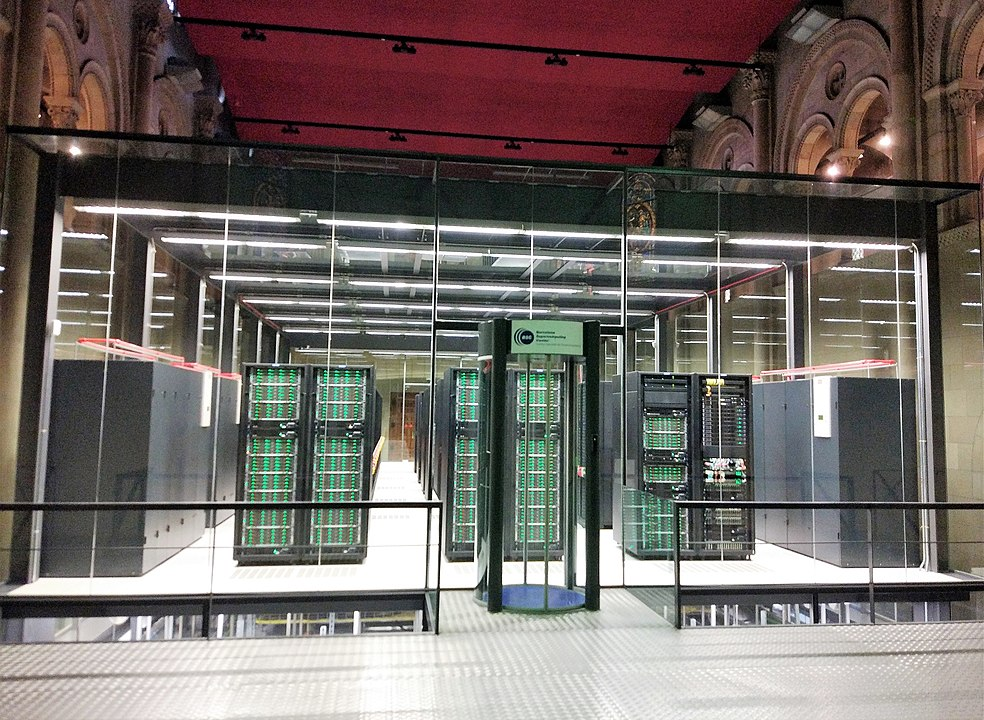
\includegraphics[width=0.6\textwidth]{mn4}
  \caption[MareNostrum4 machine]{MareNostrum 4 machine. {By Gemmaribasmaspoch, CC BY-SA 4.0, \url{https://commons.wikimedia.org/w/index.php?curid=61308843}}}
  \label{fig:mn4}
\end{figure}

\textbf{Alya}

Alya \cite{alya} is the application we will be studying.  It is code oriented to high-performance computational mechanics that aims to solve engineering coupled problems. In other words, Alya consists of multiple modules that can be joined to solve a specific problem. For this work, we will focalise the analysis into a new Alya module devoted to simulate combustion processes. We will work with a real industry use case in the combustion industry.

Alya supports a wide variety of programming models but the module we are given to analyse only supports MPI. It is contemplated to add support for other programming models if we find out that doing so improves the performance.

\textbf{Performance Analysis}

Running real use case scientific applications in supercomputer environments is crucial to identify flaws that deplete its performance when running on several machines.

Performance analysis refers to the process of gathering data from application executions, study the data and finally identify bottlenecks of the program.

In the state-of-the-art performance analysis, there is a wide variety of methodologies. However, this work is under the POP Center of Excellence resultantly we chose its methodology  \cite{popMethod}. The application of the methodology is tricky,  \cite{paperparaver} shows the application of the methodology.

\textbf{BSC tools}

As said, for a performance analysis we need data about the execution of programs and tools to visualize the data to get an insight of the bottlenecks.

The main BSC tools we are going to use are:

\begin{itemize}
  \item \textbf{Extrae} \cite{extraeTools}: This is the central tool of all the collection of tools. It allows the user to hook up Extrae to the application and gather data during the execution. We can trace events such as the MPI calls, PAPI \cite{papi}  counters, other programming models events and even manually instrument the code using Extrae API. All the data extracted is dumped into a file we call trace.
  \item \textbf{Basic Analysis} is a set of scripts that using existing BSC tools automatically computes the POP methodology metrics.
  \item \textbf{Paraver} \cite{paraverPaper} \cite{paraverWeb} is a powerful desktop application that allows to load up traces and study them. The two main ways to study a trace are using a histogram or a timeline. Histograms allow to study the tendency of some certain counter in the execution. Figure \ref{fig:hist} shows an example histogram where the \textit{y-axis} shows MPI-processes and the \textit{x-axis} shows different frequency values. The color represents how frequent is that frequency value during the execution, green is not frequent and blue is frequent. Time-lines allow to analyse the behaviour of the code in certain regions. For example, the pattern of MPI calls, the memory access patterns, the executions of tasks on a shared-memory programming model. Figure \ref{fig:trace} shows a time-line where \textit{y-axis} show MPI-processes and \textit{x-axis} show time. The color of a process at a certain time show what the process is doing. Blue means the process is computing something useful while black means the process is idle, communicating or in a synchronization. Looking at traces in the Paraver UI it is not the best visual appealing experience. For the sake of comprehensiveness we will use tracedraw \cite{tracedraw} package for drawing more visual appealing traces. Figure \ref{fig:tracedraw} shows the imitation of Figure \ref{fig:trace} with tracedraw.

    \begin{figure}[htbp]
      \centering
      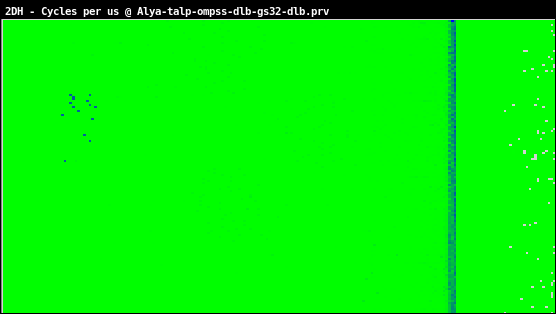
\includegraphics[width=0.8\textwidth]{sample_histogram}
      \caption[Sample Paraver Histogram]{Sample Paraver Histogram. Own compilation.}
      \label{fig:hist}
    \end{figure}

    \begin{figure}[htbp]
      \centering
      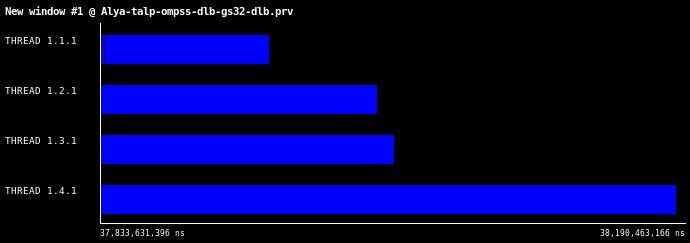
\includegraphics[width=0.8\textwidth]{sample_trace}
      \caption[Sample Paraver trace]{Sample Paraver trace. Own compilation}
      \label{fig:trace}
    \end{figure}

    \begin{figure}[htbp]
      \centering
      \begin{tracedraw}{0.8}
        \tracedrawAddToLegend(\large{Not-useful}, red)
        \tracedrawAddToLegend(\large{Useful}, blue)
        \tracedrawEnableLineName(\large{Process})
        \tracedrawSetLegendColorScale(0.5)

        \tracedrawSetLineHeight(0.5)
        \tracedrawAddChunk[color=gray, fill=blue](99)
        \tracedrawAddChunk[color=gray, fill=red](1)

        \tracedrawNewLine

        \tracedrawAddChunk[color=gray, fill=blue](50)
        \tracedrawAddChunk[color=gray, fill=red](50)

        \tracedrawNewLine
        
        \tracedrawAddChunk[color=gray, fill=blue](45)
        \tracedrawAddChunk[color=gray, fill=red](55)

        \tracedrawNewLine
        
        \tracedrawAddChunk[color=gray, fill=blue](30)
        \tracedrawAddChunk[color=gray, fill=red](70)

      \end{tracedraw}
      \caption[Sample trace representation with tracedraw]{Sample trace representation with tracedraw. Own compilation}
      \label{fig:tracedraw}
    \end{figure}

\end{itemize}


\subsubsection{Problem to be resolved}
This project is motivated by the Propulsion Technologies BSC group applying to a POP Performance Analysis assessment.

The problem to solve is that the combustion module they programmed is slow. We are asked to find out why and if possible, apply optimizations and modifications to the code to improve its performance and efficiency. In Section \ref{sec:objectives} we will discuss the solutions to the problem by defining our objectives.


\subsubsection{Stakeholders}


The following groups will benefit from the work.

\textbf{Propulsion Technologies BSC group}

This is the principal stakeholder as it is the developer of the module and the applicant for the analysis.

\textbf{Scientific community}

This beneficiary is also benefited from the work since the results and conclusions of the study are public and open to the scientific community. More in detail, the combustion community will be benefited as the results of the study and the possible optimizations will be shared and used in the newly approved Center of Excellence in Combustion (CoEC)\footnote{\url{https://www.bsc.es/news/bsc-news/the-ec-approves-two-new-centres-excellence-high-performance-computing-applications-led-bsc}}. 

\textbf{Society}

POP is an European Center of Excellence, this means that the European Union states that the work done under the Center of Excellence (POP) will have a positive impact to the European Society.

In the case of optimizing the combustion module it will impact because combustion researchers will be able to simulate faster which can lead to new discoveries on more energy efficient and pollute less combustions.

Optimizing a code also implies that the application users will use less time the machine which means that they will use less energy for their research.
